\section{Entrega 3}


\subsection{Objetivo}


El objetivo de esta entrega es diseñar e incluir en el proyecto todos los escenarios y entornos necesarios para el juego. El proyecto cuenta con un escenario principal donde transcurre la mayoría del juego, así como varios escenarios de menor tamaño y complejidad que se utilizarán en cada una de las distintas pruebas.



\subsection{Iteración 1}

En esta iteración se han diseñado todos los escenarios en los que se desarrolla el proyecto.  El primer paso es decidir como se conectarán los escenarios entre sí. 

La primera opción consiste en mantener cada escenario aislado del resto, haciendo que el jugador comience en el principal y sea transportado al escenario correspondiente a cada prueba cuando vaya a realizarla, siendo transportado de nuevo al escenario principal al completarla. Esta aproximación permite una mayor diferenciación y caracterización de cada escenario, pero puede resultar poco inmersiva ya que el jugador se ve transportado constantemente sin importar sus acciones.

La segunda opción mantiene todos los escenarios unidos entre sí en todo momento, haciendo que los escenarios de las pruebas formen parte del principal, esto aumenta enormemente la inmersión de usuario ya que todos los elementos del juego están a la vista y no hay movimientos de cámara ni posición ajenos al jugador. Con este enfoque se consigue más realismo y al mismo tiempo se reduce el tamaño y la carga de trabajo asociada a cada escenario, ya que las pruebas no necesitarán un entorno completo, si no que se reutiliza gran parte del escenario principal. 

Finalmente, por los motivos ya expuestos, se decide utilizar la segunda opción y crear un escenario principal que contenga diferentes partes para cada prueba.

Este proyecto toma prestadas muchas ideas y conceptos de los concursos televisivos, por lo que son una fuente de inspiración ideal para la estética y el diseño de los escenarios (véanse figuras \ref{fig:E3_ahoraCaigo} y \ref{fig:E3_atrapaMillon}).

\begin{figure}
  \centering
    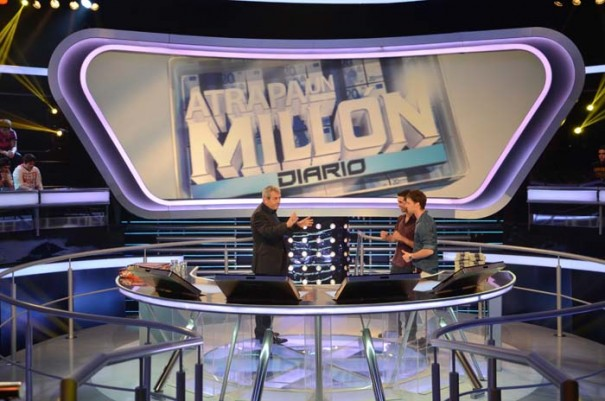
\includegraphics[width=0.7\textwidth]{04.Desarrollo/03.Entrega3/01.Iteracion3_1/00.Figuras/01.atrapa_un_millon.jpg}
    \caption{Plató del programa de televisión 'Atrapa un millón'. \cite{AI_img_atrapaMillon}}
    \label{fig:E3_atrapaMillon}
\end{figure}

\begin{figure}
  \centering
    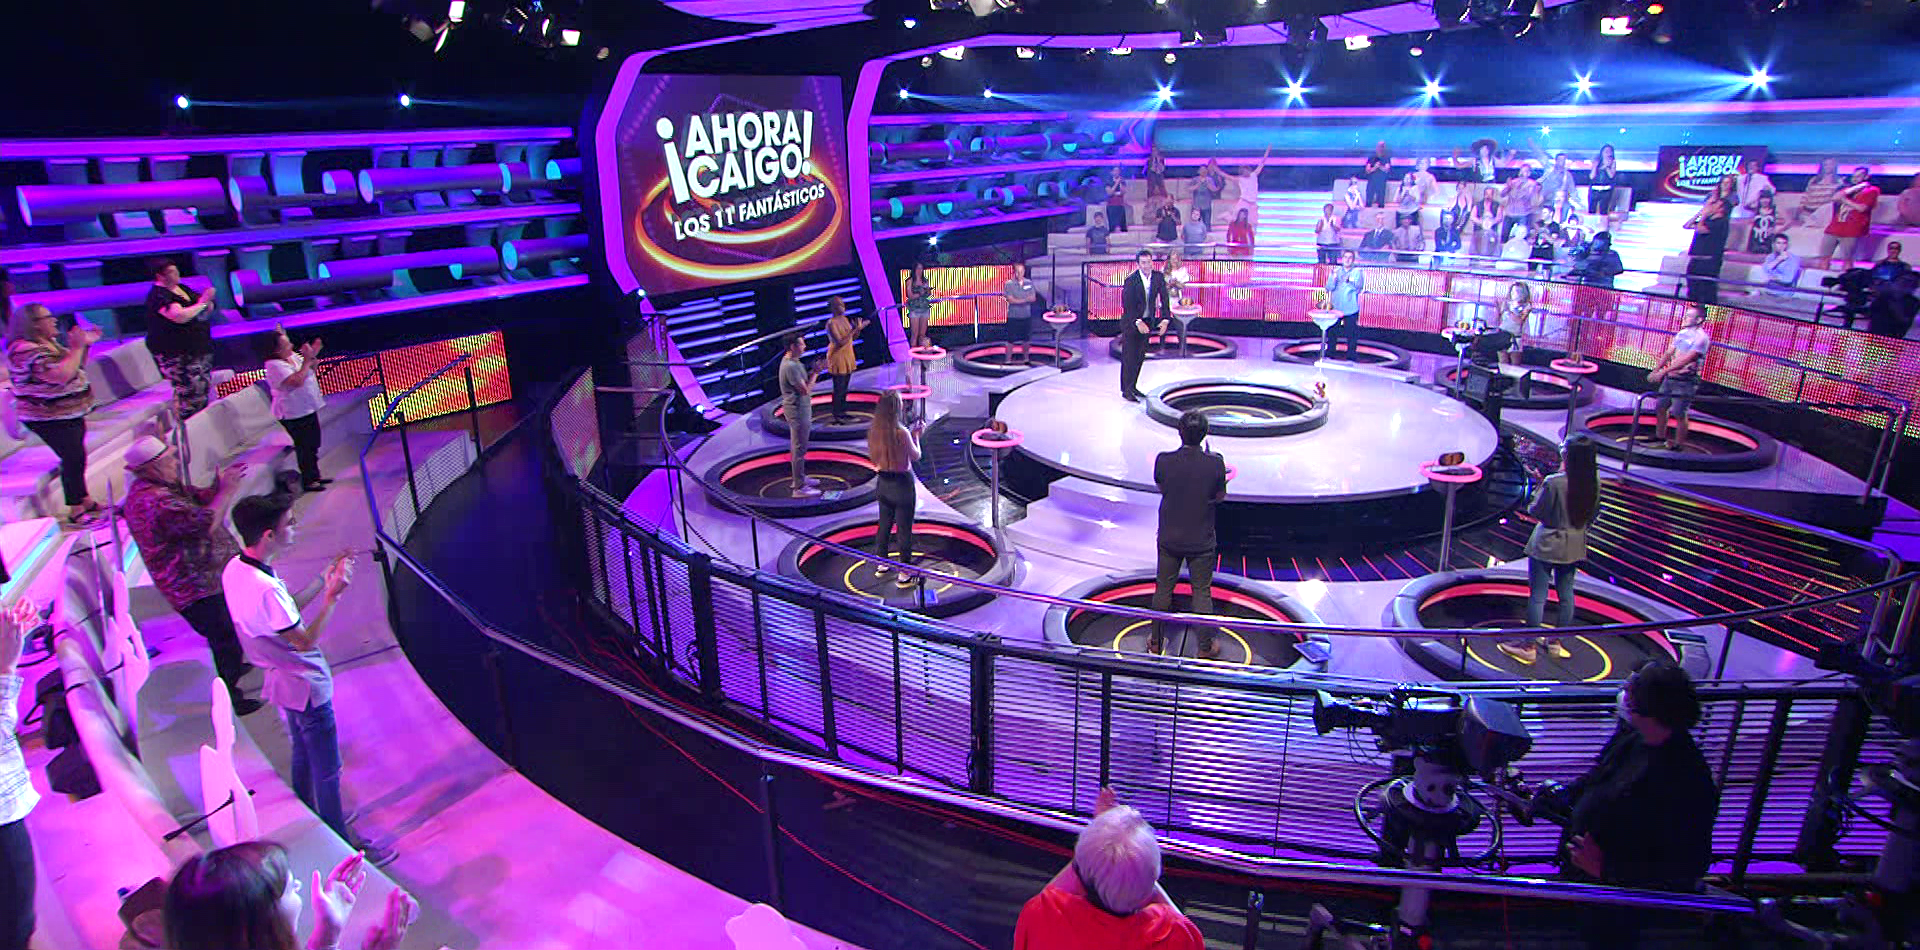
\includegraphics[width=0.7\textwidth]{04.Desarrollo/03.Entrega3/01.Iteracion3_1/00.Figuras/02.ahora_caigo.png}
    \caption{Plató del programa de televisión '¡Ahora caigo!'. \cite{AI_img_ahoraCaigo}}
    \label{fig:E3_ahoraCaigo}
\end{figure}




Como se muestra en las figuras \ref{fig:E3_escenarioArriba} y \ref{fig:E3_escenarioPerfil}, el escenario principal será circular, con el jugador situado en el centro. En los alrededores del habrá gradas con público (coloreadas de azul en las figuras), excepto en un trozo en el que se situará una pantalla gigante en la que se presentará información al jugador (rectángulo superior). En este caso, se ha designado una zona del escenario que es intercambiable (rayada en negro en las figuras), y en dicha zona aparecerá el escenario adecuado para cada prueba subiendo desde el suelo hasta la posición del jugador de forma similar a algunos elevadores en escenarios de espectáculos. Finalmente, la zona verde en las figuras contendrá elementos típicos de un plató de televisión como focos y altavoces, y su objetivo es encuadrar la zona donde transcurren las pruebas y se da información importante al jugador.


\begin{figure}
  \centering
    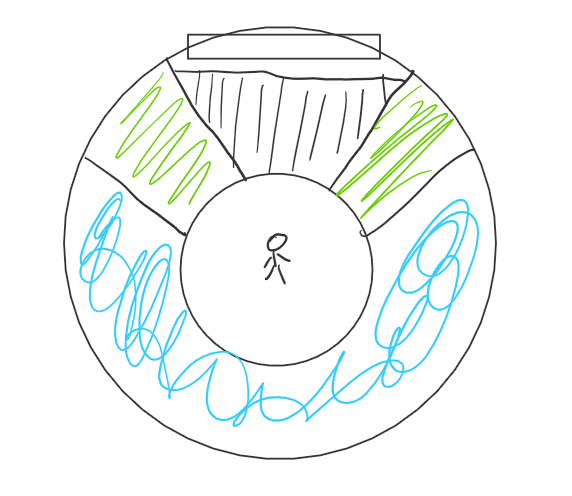
\includegraphics[width=0.5\textwidth]{04.Desarrollo/03.Entrega3/01.Iteracion3_1/00.Figuras/03.boceto_escenario_arriba.png}
    \caption{Boceto de la vista superior del escenario principal. En azul la zona de público, en verde la zona de atrezo, en negro la parte intercambiable para las pruebas.}
    \label{fig:E3_escenarioArriba}
\end{figure}

\begin{figure}
  \centering
    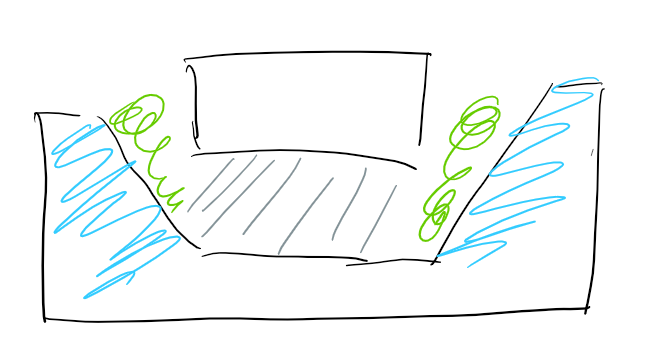
\includegraphics[width=0.5\textwidth]{04.Desarrollo/03.Entrega3/01.Iteracion3_1/00.Figuras/04.boceto_escenario_perfil.png}
    \caption{Boceto de la vista de perfil del escenario principal. En azul la zona de público, en verde la zona de atrezo, en negro la parte intercambiable para las pruebas.}
    \label{fig:E3_escenarioPerfil}
\end{figure}

Para la zona intercambiable del escenario que contendrá los distintos decorados, se ha buscado llenarla de objetos y atrezo relacionado con la prueba correspondiente, de forma que, al comenzar una prueba, aparecerá desde abajo todo el decorado y objetos necesarios para realizar dicha prueba. Tras finalizar la prueba, el escenario vuelve a su configuración original. Por tanto, solo es necesario diseñar un trozo pequeño del escenario para cada tipo de prueba.

Por lo general, las pruebas se pueden dividir en dos según el uso de su escenario: las que utilizan la pantalla principalmente y el resto es decoración, y las que utilizan los objetos virtuales del escenario como parte de la prueba y la pantalla sirve de decoración.


\subsubsection{Pruebas de pantalla}

Estas son las pruebas que utilizarán principalmente la pantalla y el resto del escenario contendrá objetos decorativos acordes con el tipo de prueba. La prueba de baile (figura \ref{fig:E3_baile}) utiliza la pantalla para mostrar al jugador los movimientos que tiene que realizar en cada momento, en este caso el escenario contendrá objetos como instrumentos musicales, tocadiscos, o una persona bailando.

\begin{figure}
  \centering
    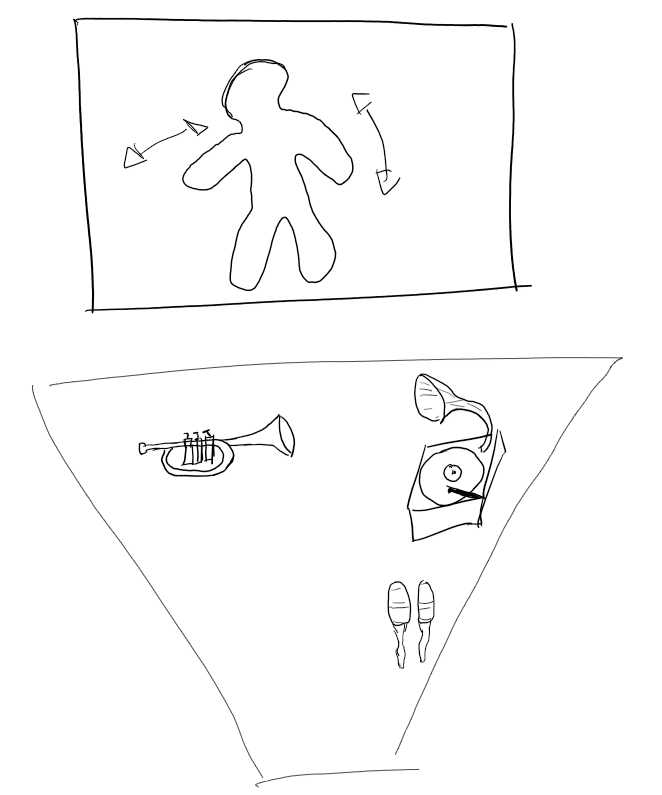
\includegraphics[width=0.5\textwidth]{04.Desarrollo/03.Entrega3/01.Iteracion3_1/00.Figuras/05.baile.png}
    \caption{Boceto del escenario para la prueba de baile.}
    \label{fig:E3_baile}
\end{figure}

La prueba de turismo también es de este tipo. En la pantalla de muestra una imagen de un monumento o lugar famoso que el jugador debe descubrir mientras que el resto del escenario se llena con objetos referentes a los viajes, como se muestra en la figura \ref{fig:E3_turismo}.

\begin{figure}
  \centering
    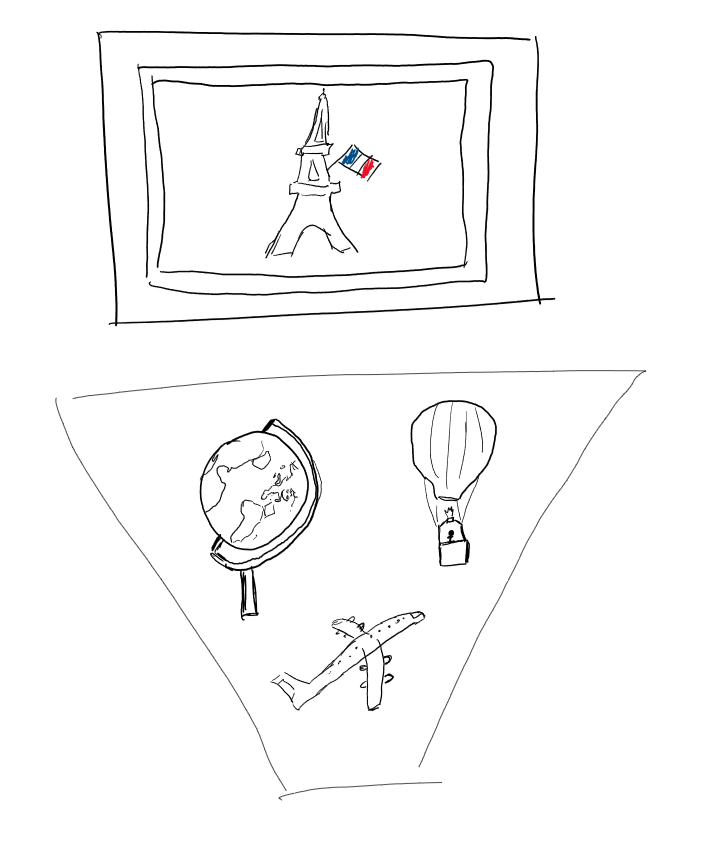
\includegraphics[width=0.5\textwidth]{04.Desarrollo/03.Entrega3/01.Iteracion3_1/00.Figuras/06.turismo.png}
    \caption{Boceto de la decoración para la prueba de turismo. En la pantalla una imagen de la torre Eiffel, con decorado de viajes: avión, globo terráqueo y globo aerostático.}
    \label{fig:E3_turismo}
\end{figure}


En las pruebas de situaciones y descripciones se sigue el mismo diseño, en la pantalla se muestra una imagen o situación que el jugador debe comentar. Pero estás pruebas podrían ser del segundo tipo y usar el escenario en lugar de la pantalla si la situación a describir es una que se puede representar con objetos virtuales animados en lugar de una foto o video en la pantalla.

La prueba de adivinar la canción es un caso especial, ya que, tratándose de sonido, no es necesario el uso de la pantalla, pero de igual forma se puede decorar el escenario como se muestra en la figura \ref{fig:E3_cancion}.

\begin{figure}
  \centering
    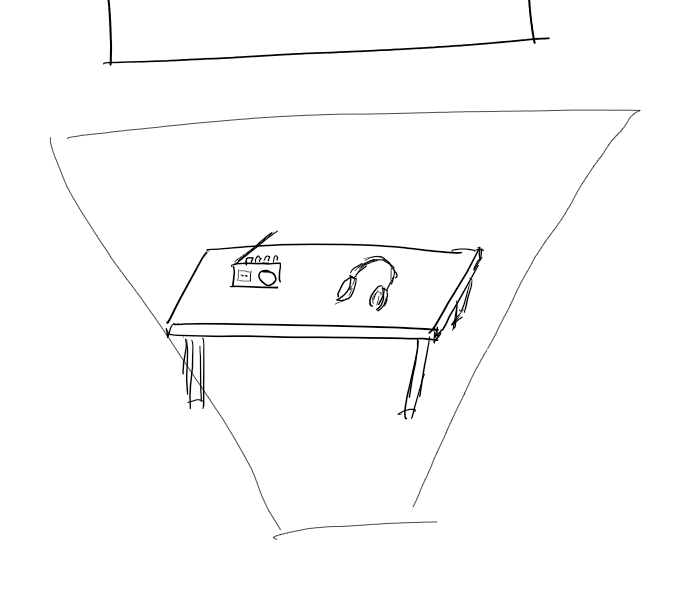
\includegraphics[width=0.5\textwidth]{04.Desarrollo/03.Entrega3/01.Iteracion3_1/00.Figuras/07.cancion.png}
    \caption{Boceto de la decoración para la prueba de adivinar la canción.}
    \label{fig:E3_cancion}
\end{figure}

Finalmente, en la prueba de superposición de objetos, se mostrará una imagen en la pantalla y el jugador tendrá que discernir de qué objetos se trata. Para facilitar esta tarea es sería posible que en el escenario aparecieran varios objetos virtuales, entre ellos los que se encuentran superpuestos en la imagen de la pantalla.



\subsubsection{Pruebas de escenario}

Estas son aquellas pruebas que dependen de los objetos del escenario y requieren su interacción para ser completadas, dejando a la pantalla el papel de decoración.

La prueba de figuras, en la que el usuario debe adoptar una posición que se le muestra antes de que se acabe el tiempo, utiliza un objeto que imita a un recortable de cartón o espantapájaros de una silueta posando. Dicha silueta se moverá hacia el usuario y este debe haber adoptado la posición correcta cuando la silueta llegue al jugador. El funcionamiento de esta prueba aparece bocetado en la figura \ref{fig:E3_figuras}.


\begin{figure}
  \centering
    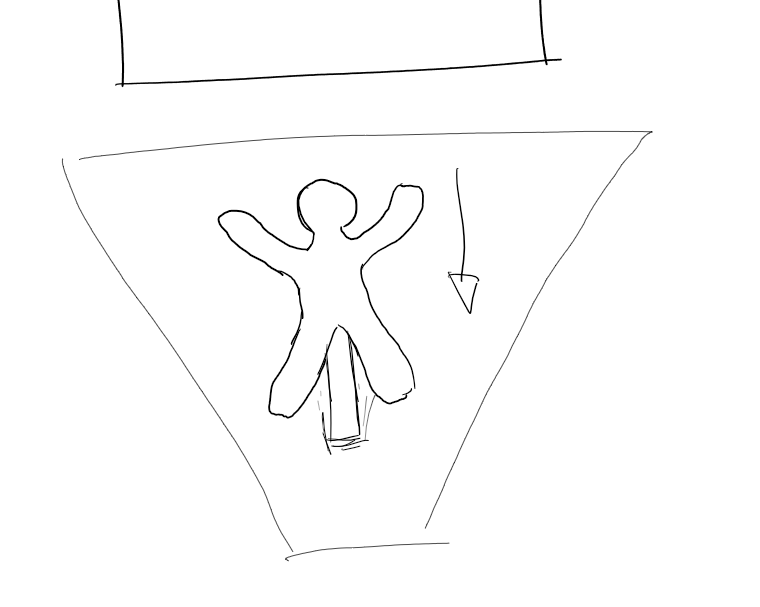
\includegraphics[width=0.5\textwidth]{04.Desarrollo/03.Entrega3/01.Iteracion3_1/00.Figuras/08.figuras.png}
    \caption{Boceto para la prueba de figuras, con una silueta acercándose al jugador.}
    \label{fig:E3_figuras}
\end{figure}

Para la prueba de objetivos, en la que el jugador debe tocar objetos que se mueven hacia él, el escenario utilizado solo contendrá dichos objetos en movimiento, como se pueden ver en el boceto de la figura \ref{fig:E2_objetivos}.



Para la prueba de asociación de sonidos únicamente se presenta ante el jugador una mesa en la que aparece un grupo de distintos objetos y el jugador debe seleccionar cual está produciendo el sonido mediante botones colocados frente a cada objeto (figura \ref{fig:E3_sonidos}). De forma similar, la prueba de agrupación de objetos también utiliza solo una mesa con un grupo de objetos, en este caso tiene también dos zonas donde agrupar los objetos por sus categorías (figura \ref{fig:E3_agrupacion}).

\begin{figure}
  \centering
    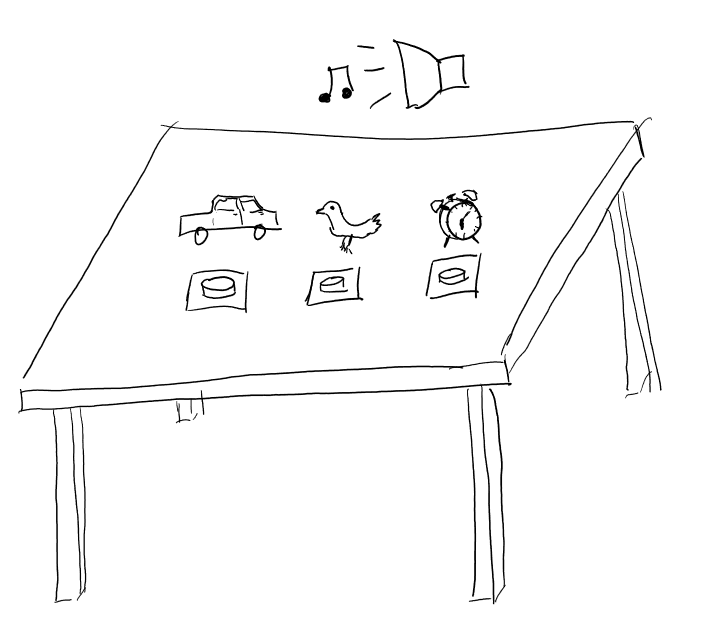
\includegraphics[width=0.5\textwidth]{04.Desarrollo/03.Entrega3/01.Iteracion3_1/00.Figuras/09.sonidos.png}
    \caption{Boceto con la mesa para la prueba de asociación de sonidos. Presenta distintos objetos con botones que corresponde a cada uno.}
    \label{fig:E3_sonidos}
\end{figure}

\begin{figure}
  \centering
    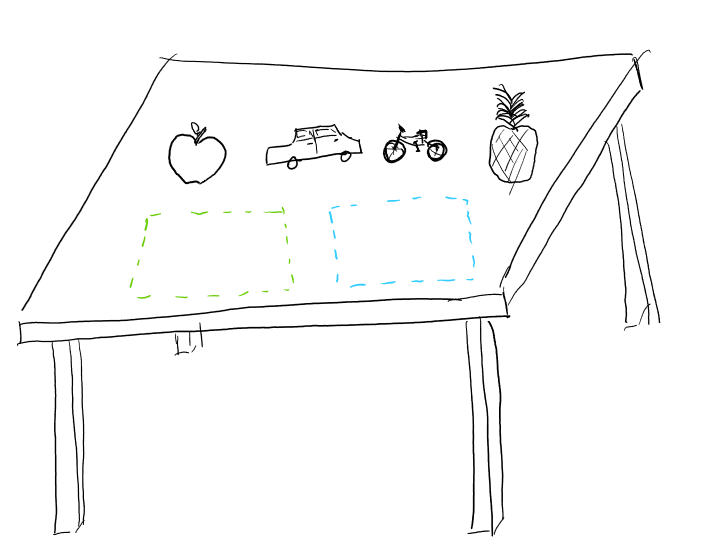
\includegraphics[width=0.5\textwidth]{04.Desarrollo/03.Entrega3/01.Iteracion3_1/00.Figuras/10.agrupacion_objetos.png}
    \caption{Boceto para la prueba de asociación de objetos, mostrando dos zonas (verde y azul) para la clasificación de los objetos.}
    \label{fig:E3_agrupacion}
\end{figure}


Por último, está la prueba de localización de sonidos, en este caso el escenario a utilizar es el propio escenario principal, ya que la prueba consiste en colocar una fuente de sonido en un punto del espacio y que el jugador se gire hasta encontrarla. De este modo se puede aprovechar el amplio espacio del escenario para colocar la fuente como se ve en la figura \ref{fig:E3_localizacionSonido}.

\begin{figure}
  \centering
    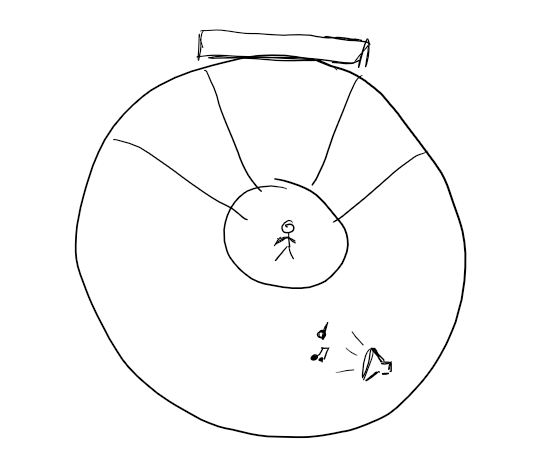
\includegraphics[width=0.5\textwidth]{04.Desarrollo/03.Entrega3/01.Iteracion3_1/00.Figuras/11.localizacion_sonido.png}
    \caption{Boceto de la vista cenital del escenario principal, mostrando una posible colocación de la fuente de sonido para la prueba de localización de sonidos.}
    \label{fig:E3_localizacionSonido}
\end{figure}






\subsection{Iteración 2}

En esta iteración se procede a la creación de los distintos escenarios y decorados para el proyecto. Para esto se puede utilizar cualquier software de modelado 3D, incluso el propio Unity. Se ha elegido utilizar Blender, una herramienta totalmente gratuita y de las más potentes del mercado.


\subsubsection{Escenario principal}

Todas las partes básicas del escenario se han creado en Blender como un único elemento formado internamente por distintas partes. Se ha comenzado creando una plataforma circular donde estará el usuario, a la cual se le ha añadido un suelo inferior también circular. Para completar la parte central de escenario (figura \ref{fig:E3_escenarioCentral}), se añaden unas gradas en la mitad posterior del círculo. Para crear las gradas se ha recurrido a la técnica de revolución de un perfil, que consiste en diseñar únicamente el perfil del objeto deseado y posteriormente hacerlo girar sobre un eje para crear un objeto en la zona que barre el perfil.

\begin{figure}
  \centering
    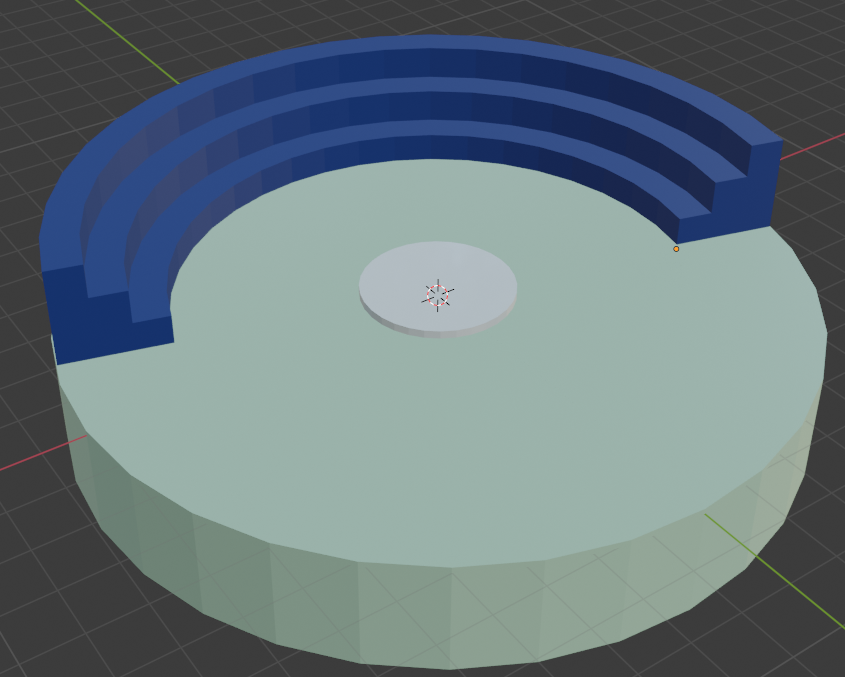
\includegraphics[width=0.5\textwidth]{04.Desarrollo/03.Entrega3/02.Iteracion3_2/00.Figuras/01.escenario_5.png}
    \caption{Parte central del escenario.}
    \label{fig:E3_escenarioCentral}
\end{figure}

Como parte del proceso continuo de mejora del proyecto, se decide que determinadas pruebas transcurran en una zona concreta del escenario con una ambientación más adecuada. Estas pruebas son las que conllevan amplios movimientos del usuario: baile, posiciones, parada y objetivos, por eso, la ambientación de esta nueva zona consistirá en colocar un escenario de baile desde el cual recibirá la prueba el jugador. Se añade también una pared para encapsular el escenario dentro del espacio virtual (figura \ref{fig:E3_escenario2}).


\begin{figure}
  \centering
    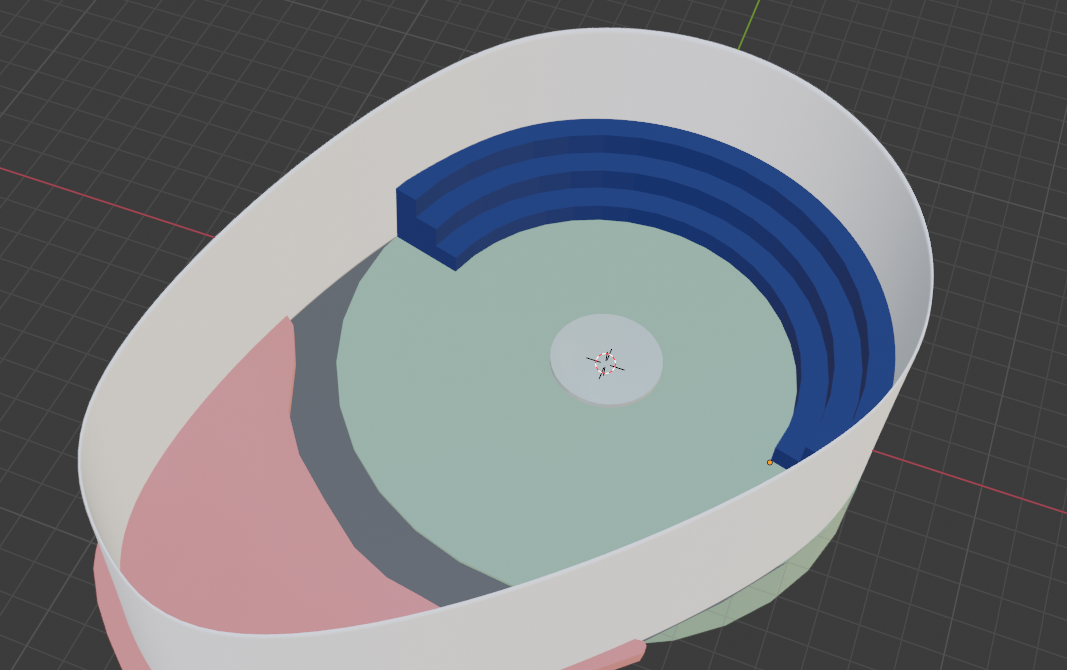
\includegraphics[width=0.5\textwidth]{04.Desarrollo/03.Entrega3/02.Iteracion3_2/00.Figuras/02.escenario_6.png}
    \caption{Plataforma principal con el escenario de baile y las paredes que rodean todo el perímetro.}
    \label{fig:E3_escenario2}
\end{figure}

En el siguiente paso en la creación de la base para el escenario de juego, se añade una pantalla para que el jugador pueda recibir información mediante texto e imágenes, un pequeño pedestal frente al escenario donde el jugador se trasladará para realizar las pruebas pertinentes, y finalmente se ha recortado un agujero en el suelo del escenario por donde bajarán y subirán los decorados de cada prueba individual. Estos cambios se pueden apreciar en la figura \ref{fig:E3_escenario3}.

\begin{figure}
  \centering
    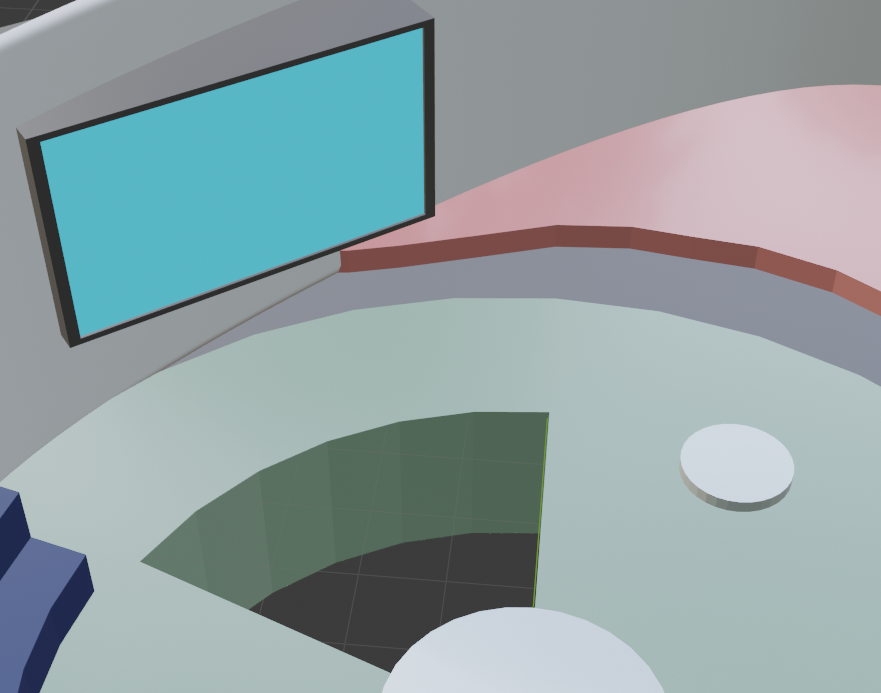
\includegraphics[width=0.5\textwidth]{04.Desarrollo/03.Entrega3/02.Iteracion3_2/00.Figuras/03.escenario_7.png}
    \caption{Detalle de la colocación de la pantalla, el pedestal secundario y el hueco del ascensor.}
    \label{fig:E3_escenario3}
\end{figure}


Finalmente se construye el ascensor que ocupará el hueco y se usará como base para el decorado de las pruebas individuales. Para ello se ha diseñado un ascensor modular que puede adaptarse a las necesidades de cada prueba, pudiendo ser utilizado en su forma básica: proporcionando únicamente un suelo (figura \ref{fig:E3_ascensorVacio}); llevando integrada una mesa en la que aparecerán objetos con los que el jugador podrá interactuar (figura \ref{fig:E3_ascensorMesa}); o con una extensión para la mesa que permite colocar mayor cantidad de objetos en ella (figura \ref{fig:E3_ascensorMesaExtendida}).


\begin{figure}
\centering
\begin{minipage}{.3\textwidth}
  \centering
  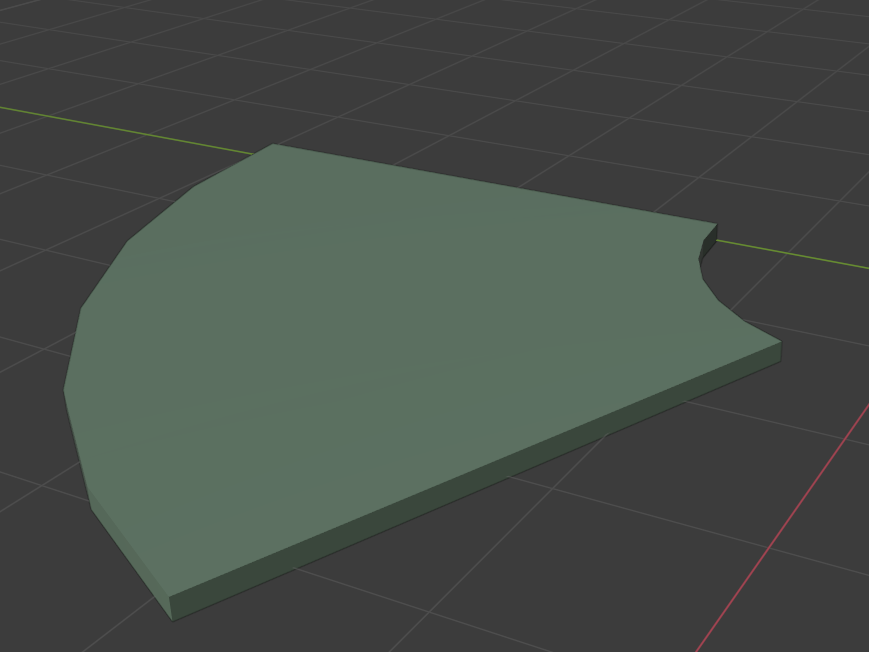
\includegraphics[width=.9\linewidth]{04.Desarrollo/03.Entrega3/02.Iteracion3_2/00.Figuras/04.ascensor_3.png}
  \captionof{figure}{Ascensor simple.}
  \label{fig:E3_ascensorVacio}
\end{minipage}%
\begin{minipage}{.3\textwidth}
  \centering
  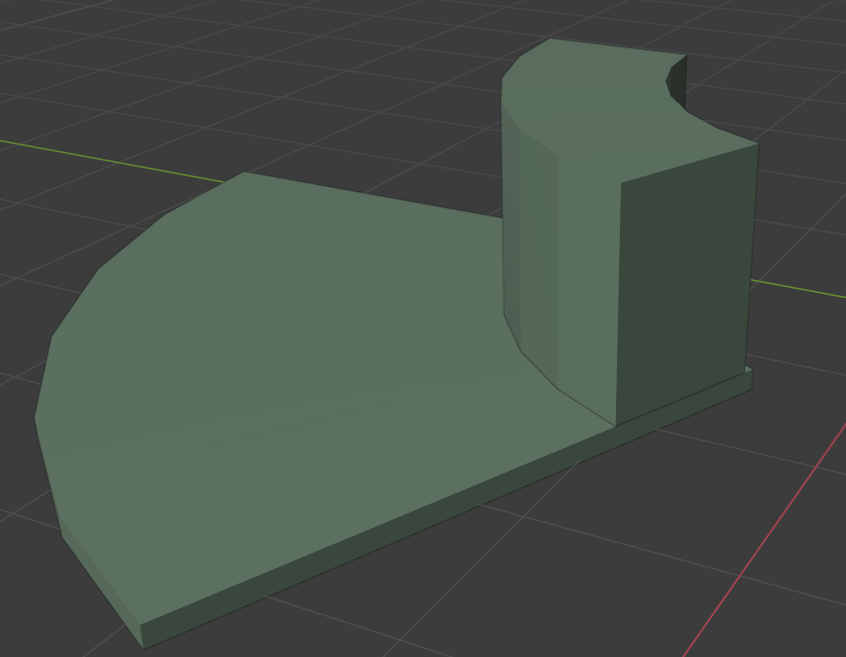
\includegraphics[width=.87\linewidth]{04.Desarrollo/03.Entrega3/02.Iteracion3_2/00.Figuras/05.ascensor_2.png}
  \captionof{figure}{Ascensor con mesa.}
  \label{fig:E3_ascensorMesa}
\end{minipage}
\begin{minipage}{.3\textwidth}
  \centering
  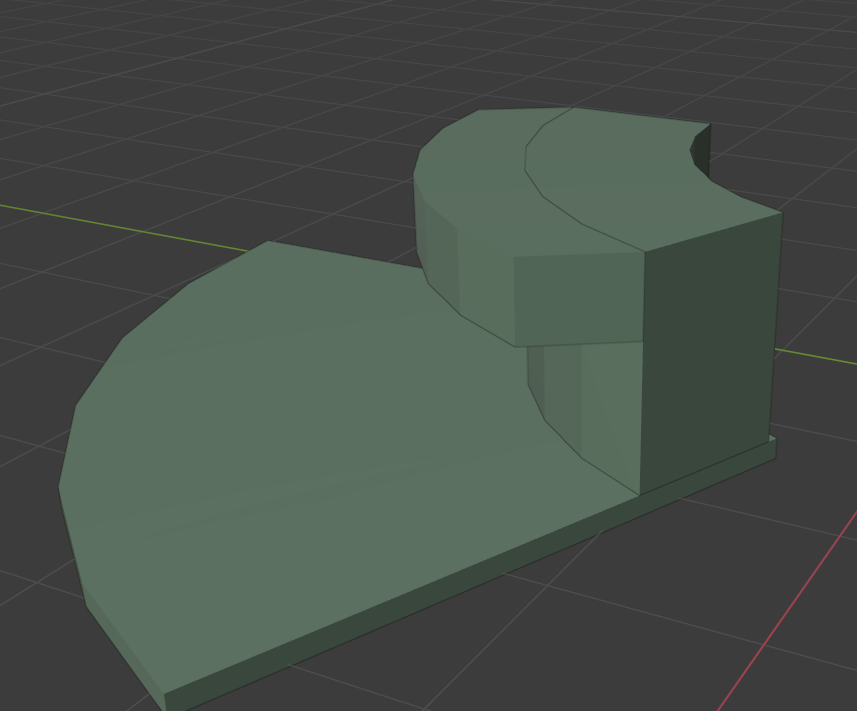
\includegraphics[width=.77\linewidth]{04.Desarrollo/03.Entrega3/02.Iteracion3_2/00.Figuras/06.ascensor_1.png}
  \captionof{figure}{Ascensor con mesa extendida.}
  \label{fig:E3_ascensorMesaExtendida}
\end{minipage}
\end{figure}





\subsubsection{Escenarios secundarios}


El decorado de los escenarios secundarios consta de una mezcla de objetos creados en Blender y una serie de objetos que ofrece Asset Store, la plataforma oficial de Unity para la distribución de contenido para ser utilizado en diversos proyectos. 

Para las pruebas de movimiento, hay que decorar el escenario de baile, para esto se han utilizado modelos de distintos instrumentos musicales (guitarra, piano, bajo y trompeta), así como un micrófono. Para dar vida a los músicos se ha utilizado un modelo de humano caricaturizado, que además se utilizará para representar todos los movimientos que el jugador necesita realizar. Por último, se han añadido unas estructuras de iluminación y varios focos en la parte superior del escenario. Véase figura \ref{fig:E3_escenarioBaile}.

\begin{figure}
  \centering
    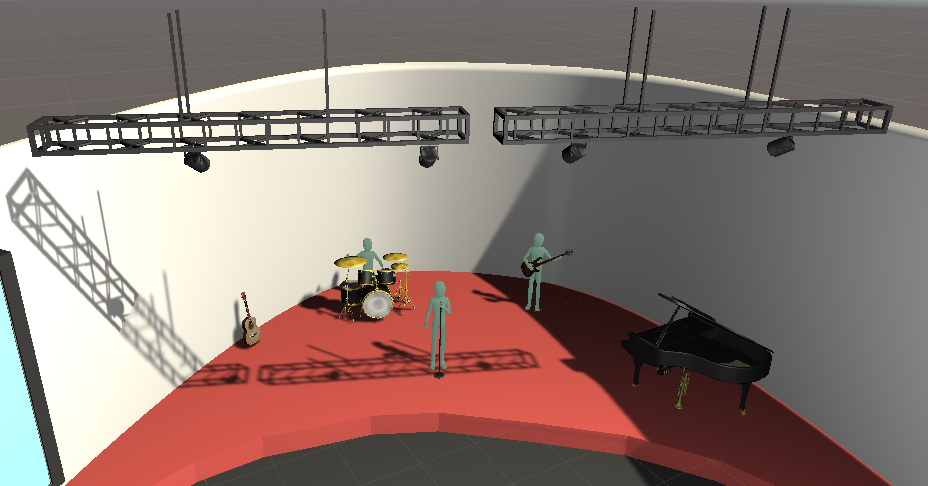
\includegraphics[width=0.5\textwidth]{04.Desarrollo/03.Entrega3/02.Iteracion3_2/00.Figuras/07.unity_1.png}
    \caption{Vista del escenario de baile completo.}
    \label{fig:E3_escenarioBaile}
\end{figure}

Además, para la prueba de objetivos se han creado dos cubos biselados en colores azul y rojo (figura \ref{fig:E3_modelosObjetivos}) que representarán los objetivos que el jugador debe golpear.

\begin{figure}
  \centering
    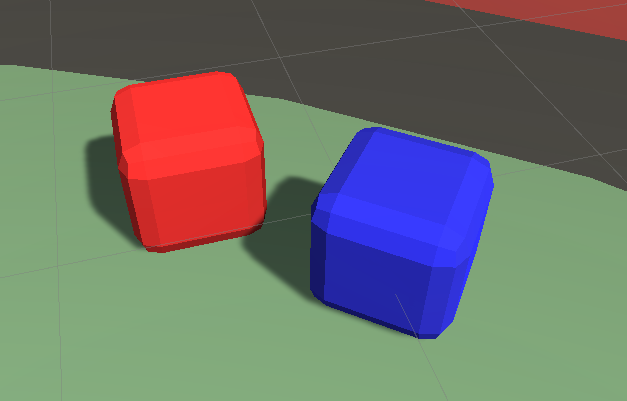
\includegraphics[width=0.5\textwidth]{04.Desarrollo/03.Entrega3/02.Iteracion3_2/00.Figuras/08.unity_5.png}
    \caption{Modelos para los objetivos que el jugador debe golpear.}
    \label{fig:E3_modelosObjetivos}
\end{figure}

El decorado para la prueba de turismo utiliza el ascensor sin mesa y adorna el espacio entre el jugador y la pantalla con objetos de temática viajera. En este caso como se ve en la figura \ref{fig:E3_escenarioTurismo}, se han colocado un globo aerostático, un avión de pasajeros despegando y en el centro un globo terráqueo.


\begin{figure}
  \centering
    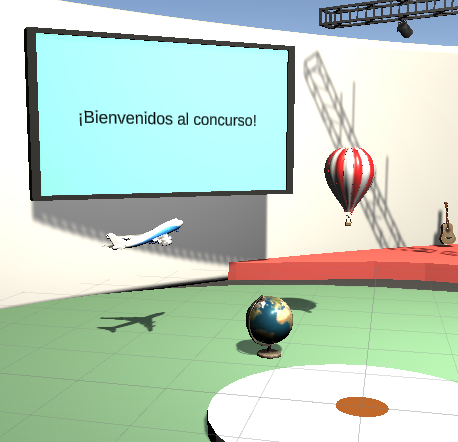
\includegraphics[width=0.5\textwidth]{04.Desarrollo/03.Entrega3/02.Iteracion3_2/00.Figuras/09.unity_2.png}
    \caption{Presentación del decorado para la prueba de turismo.}
    \label{fig:E3_escenarioTurismo}
\end{figure}


Para la prueba donde el jugador debe adivinar una canción que está sonando se ha utilizado el ascensor con mesa, en la cual se han colocado varios objetos del mundo de la música (figura \ref{fig:E3_escenarioCancion}). En el centro se han colocado unos auriculares de diadema, mientras que a cada uno de sus lados hay un dispositivo cuyo uso es reproducir música: un tocadiscos y una radio. Se han elegido objetos de estética antigua ya que resultarán más familiares al público objetivo de este proyecto, que son las personas mayores.

\begin{figure}
  \centering
    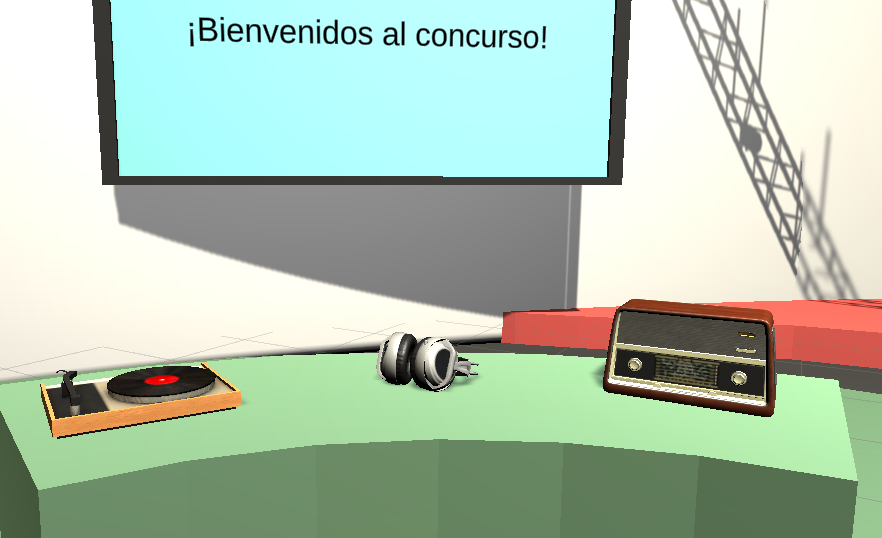
\includegraphics[width=0.5\textwidth]{04.Desarrollo/03.Entrega3/02.Iteracion3_2/00.Figuras/10.unity_3.png}
    \caption{Mesa con decorado para la prueba de adivinar la canción.}
    \label{fig:E3_escenarioCancion}
\end{figure}

El resto de las pruebas utilizan objetos virtuales para su realización, por lo que la inclusión de objetos decorativos similares podría llevar a confusión, por ejemplo, en la prueba de agrupación de objetos. Aun así, se seguirá utilizando el patrón ya marcado de utilizar los tres tipos de ascensor diseñados, pero en lugar de contener decorado, contendrán los objetos necesarios para las pruebas.

Para finalizar la decoración del escenario general y generar un ambiente más acogedor para el jugador, se han poblado las gradas con modelados caricaturizados como los músicos del escenario de baile (figura \ref{fig:E3_escenarioPublico}).


\begin{figure}
  \centering
    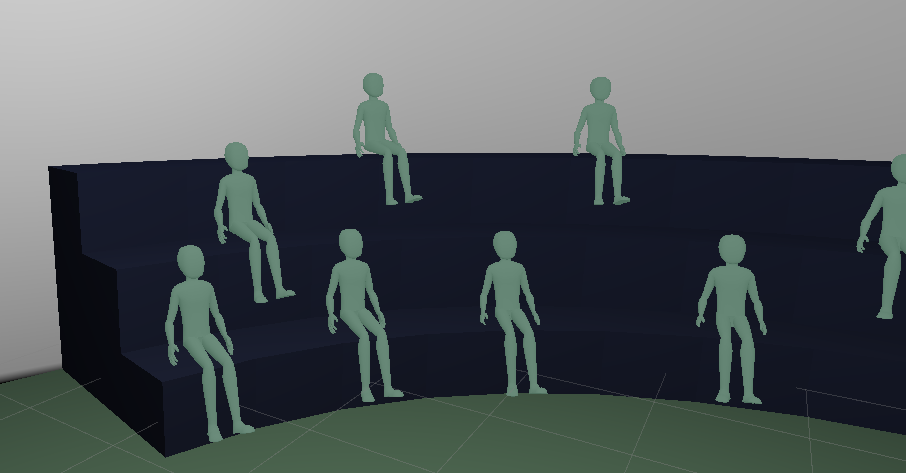
\includegraphics[width=0.5\textwidth]{04.Desarrollo/03.Entrega3/02.Iteracion3_2/00.Figuras/11.unity_4.png}
    \caption{Presentación de las figuras que actúan como público.}
    \label{fig:E3_escenarioPublico}
\end{figure}






\subsection{Iteración 3}


En esta última iteración para esta entrega se busca conocer la respuesta de varios usuarios ante los escenarios desarrollados. Parte de esta iteración se ha realizado en paralelo a la anterior, durante el desarrollo de los escenarios. Esto ha permitido realizar un trabajo más efectivo desde una fase temprana de la entrega. Esta vez solo se ha podido contar con una persona para que ofrezca su opinión y críticas sobre el trabajo desarrollado. 

Esta persona tiene entre 20 y 30 años y tiene un amplio conocimiento tecnológico pero una experiencia limitada en realidad virtual. Para la realización de la prueba se ha colocado al usuario en el centro del escenario y se le ha dado libertad de desplazamiento por todo el escenario mientras se iba conversando para obtener información útil. 

De esta prueba han surgido varios pequeños cambios que ya han sido realizados en el proyecto, la mayoría relacionados con la posición de ciertos objetos, como la pantalla que estaba demasiado alta. Pero sin duda, el factor más importante para tener en cuenta es la escala y tamaño de los objetos del mundo virtual. Es necesario que la escala del entorno sea lo más parecida a la realidad, ya que de otra forma crea situaciones incómodas como: mesas demasiado altas o bajas, modelos de personas que parecen ser gigantes, o un espacio demasiado grande y vacío.

Finalmente, tras tomar en consideración toda esta información, se ha ido adaptando el escenario hasta su forma final, que se puede ver en la figura \ref{fig:E3_escenarioCompleto}.


\begin{figure}
  \centering
    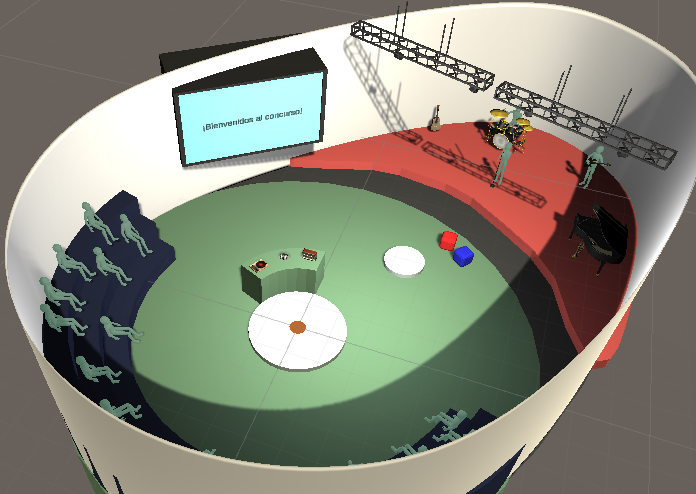
\includegraphics[width=0.5\textwidth]{04.Desarrollo/03.Entrega3/03.Iteracion3_3/00.Figuras/01.unity_6.png}
    \caption{Montaje final del escenario para la entrega 3.}
    \label{fig:E3_escenarioCompleto}
\end{figure}










\subsection{Conclusiones de la entrega}



Al igual que el desarrollo informático, la creación de arte digital es un proceso complejo y que requiere de conocimientos avanzados para obtener los resultados más realistas posibles. En este caso, para limitar la escala del proyecto ha sido necesario simplificar los diseños y utilizar objetos 3D prediseñados por otras personas, las cuales son acreditadas tanto en esta memoria como dentro del juego.

Se ha intentado recrear de forma esquemática un escenario de concurso televisivo y utilizar objetos con los cuales puedan estar familiarizados los jugadores, en este caso, mayores.

A pesar de que el entorno no es detallista, gracias a la realidad virtual, se consigue aumentar la inmersión. Esto, acompañado de las mejoras sugeridas tras algunas pruebas con personas ajenas, permite que haya una credibilidad suficiente durante el juego, y se determina que los objetos y decorados elegidos son adecuados para las pruebas a realizar y para alcanzar el objetivo de este proyecto.




